\documentclass[a4paper,12pt,headsepline]{scrartcl}

%\part{title}
\usepackage[utf8]{inputenc}
\usepackage{graphicx}
\usepackage{caption,subcaption}
\usepackage[english]{babel}
\usepackage[T1]{fontenc}
\usepackage{proof}
\usepackage{hyperref}
%\usepackage[hyphens,obeyspaces,spaces]{url}
\usepackage{fancybox}
\usepackage{amssymb,amsmath,amsthm}
\usepackage{textcomp}
\usepackage{gensymb}
\usepackage[linesnumbered,ruled,vlined,norelsize]{algorithm2e}
% \usepackage[bookmarksnumbered,hyperfootnotes=false]{hyperref} % ,pdftitle={\titleDocument}
\usepackage{color}
\usepackage{float}

\usepackage{geometry}
\geometry{left=3.5cm, right=2cm, top=2.5cm, bottom=2cm}


%test
\usepackage[backend=biber]{biblatex}
\usepackage{filecontents}

% \addbibresource{ref.bib}

\restylefloat{figure}

% Makros
\newenvironment{sketch}{\begin{proof}[Proof (Sketch)]}{\end{proof}}
\newtheorem{theorem}{Theorem}
\newtheorem{assumption}{Assumption}
\newtheorem{lemma}{Lemma}
\newtheorem{remark}{Remark}
\newtheorem{definition}{Definition}
\newtheorem{corollary}{Corollary}
\newtheorem{observation}{Observation}
\newcommand{\comment}[1]
{
	\begin{quotation}
		\textcolor{blue}{\underline{Edit:} #1}
	\end{quotation}
}
\newcommand{\TODO}[1]
{
	\begin{quotation}
		\textcolor{red}{\underline{TODO:} #1}
	\end{quotation}
}
\newcommand{\mygraphics}[3][2]{
	\begin{figure}[h]
		\centering
		\includegraphics[page=#1]{#2}
		\caption{#3}
	\end{figure}
}
% Symbols
\newcommand{\N}{\ensuremath{\mathbb{N}}}

% neue Kopfzeilen mit fancypaket
\usepackage{fancyhdr} %Paket laden
\pagestyle{fancy} %eigener Seitenstil
\fancyhf{} %alle Kopf- und Fußzeilenfelder bereinigen
\fancyhead[L]{\nouppercase{\leftmark}} %Kopfzeile links
\fancyhead[C]{} %zentrierte Kopfzeile
\fancyhead[R]{\thepage} %Kopfzeile rechts
\renewcommand{\headrulewidth}{0.4pt} %obere Trennlinie
%\fancyfoot[C]{\thepage} %Seitennummer
%\renewcommand{\footrulewidth}{0.4pt} %untere Trennlinie

\frenchspacing
\makeindex

% Pseudocode für Java
%\usepackage{listings}
%\lstset{numbers=left, numberstyle=\tiny, numbersep=5pt, keywordstyle=\color{black}\bfseries, stringstyle=\ttfamily,showstringspaces=false,basicstyle=\footnotesize,captionpos=b}
%\lstset{language=java}

% Disable single lines at the start of a paragraph (Schusterjungen)
\clubpenalty = 10000
% Disable single lines at the end of a paragraph (Hurenkinder)
\widowpenalty = 10000
\displaywidowpenalty = 10000

\begin{document}
%% das Papierformat zuerst
%\documentclass[a4paper, 11pt]{article}

% deutsche Silbentrennung
%\usepackage[ngerman]{babel}

% wegen deutschen Umlauten
%\usepackage[ansinew]{inputenc}

% hier beginnt das Dokument
%\begin{document}


\thispagestyle{empty}

%\begin{figure}[t]
% \centering
% \includegraphics[width=0.6\textwidth]{abb/logo1}
%~~~~~~~~~~
% \includegraphics[width=0.3\textwidth]{abb/logo2}
%\end{figure}


\begin{verbatim}
	
	
\end{verbatim}

\begin{center}
	\Large{Eberhard Karls Universität Tübingen}\\
	\small Wilhelm Schickard Institut Tübingen\\
\end{center}


\begin{center}
	\Large{Fachbereich Informatik}
\end{center}
\begin{verbatim}
	
	
	
	
\end{verbatim}
\begin{center}
	%\doublespacing
	\textbf{\LARGE{Minimizing the edge length ratio of planar poly-line graph drawings}}\\
	%\singlespacing
	\begin{verbatim}
		
	\end{verbatim}
	\textbf{{Arbeitsbereich Algorithmik}}
\end{center}
\begin{verbatim}
	
\end{verbatim}
\begin{center}
	
\end{center}
\begin{verbatim}
	
\end{verbatim}
\begin{center}
	\textbf{Forschungsprojekt SS21}
\end{center}
\begin{verbatim}
	
	
	
	
	
	
\end{verbatim}
\begin{flushleft}
	\begin{tabular}{llll}
		\textbf{Autor:} & & Benjamin Ulvi \c Coban & \\
		& & MatNr. 3526251 & \\
		& & \\
		\textbf{Version vom:} & & \today &\\
		& & \\
		\textbf{Betreuer:} & & Prof. Dr. Michael Kaufmann &\\
	\end{tabular}
\end{flushleft}
%\section{Introduction}
The topic of visualization of information relationships occur in various areas of work. Examples of the fields include circuit design, architecture, web science, social sciences, biology, geography, information security and software engineering. The relationships of various information is formalized \textcolor{red}{What is an undirected planar graph, what are bends, grid, poly-line, edge-length}

%\section{Preliminaries}
As otherwise mentioned, a \textit{graph} $G=(V_G,E_G)$ is a tuple consisting of two sets - the set of vertices and the set of edges. An \textit{edge} $e = (v,w), v,w \in V_G$ is a tuple and describes a connectivity relation between two vertices. Unless otherwise mentioned, the graphs are \textit{undirected}. It means that the edge $(u,v)$ is identical to the edge $(v,u)$,$u,v\in V_G$. A \textit{face} is a maximal open region of the plane bounded by edges. The degree of the graph is the amount of edges attached to it. A graph $G'$ is called a supergraph of $G$ iff $V_{G}\subseteq V_{G'}$ and $E_{G}\subseteq E_{G'}$. 
\bigskip\\
 A \textit{drawing} $\Gamma$ of a graph $G$ is a function, where each vertex is mapped on a unique point $\Gamma(v)$ in the plane and each edge is mapped on an open Jordan curve $\Gamma(e)$ ending in its vertices. A graph is \textit{planar} if and only if there exists a crossing-free representation in the plane. $G$ is maximal planar iff any further edge insertion violates the planarity property. A $k\times k$ grid is an undirected graph consisting of $k$ rows and $k$ columns of vertices. A vertex in the $i$-th row and $j$-th column is denoted as $(i,j)$.\\
 A straight line drawing on a grid of size $k\times k$ is a drawing where every vertex has its unique row and column value and every edge is drawn as a straight line. In a polyline drawing, each edge is represented by a non-empty sequence of line segments ($e = (e_1,e_2,...)$), where two consecutive line segments intersect in a unique point, a bend. Every bend lies, like the vertices, on a unique grid point.\bigskip\\
 To measure the length, the euclidian distance of a line segment is introduced as a metric. It is defined as the square root of the sum of the quadratic difference of row and column. The unit length, \UL in short, is defined as the distance between two consecutive points on the grid with either the same row or column value.\bigskip\\
 A path is a sequence of edges. A cycle is a path, so that the starting vertex and the ending vertex are identical. A tree is an acyclic graph. A graph is called connected if there is a path from every vertex to every other vertex of $G$. A $k$-ary tree is a graph where either every vertex has exactly $k$ children and one parent or is of degree 1. These are called leaves. The root of a tree is a vertex with no parent. The height of a tree is defined as the length of the longest path starting from the root. A tree is called complete, when all leaves have the same height and no further vertices can be inserted without increasing the maximum height.\bigskip\\
 A 2-terminal series-parallel graph with terminals $s,t$ is a recursively defined graph with one of the following three rules:
 \begin{enumerate}
 	\item An edge $(s,t)$ is a 2-terminal series-parallel graph
 	\item If $G_i, i = 1,2$, is a 2-terminal series-parallel graph with terminals $s_i,t_i$, then in the serial composition $t_1$ is identified with $s_2$ to obtain a 2-terminal series-parallel graph with $s_1,t_2$ as terminals
 	\item If $G_i, i=1,...,k$, is a 2-terminal series-parallel graph with terminals $s_i,t_i$, then in a parallel composition we identify all $s_i$ into one terminal $s$ and all $t_i$ into the other terminal $t$ and the result is a 2-terminal series-parallel graph with terminals $s,t$.
 \end{enumerate}
A series-parallel graph, SP-graph in short, is a graph for which every biconnected component is a 2-terminal series-parallel graph. A SP-graph is maximal if no edge can be added so while maintaining a SP-graph.\bigskip\\
A 2-tree is a recursively defined graph with at least three vertices. If $n = 3$, then the 2-tree is the $K_3$. If $n>3$, then start with a $K_3$ and every vertex added is adjacent to exactly two adjacend neighbours, forming a 3-clique. The class of 2-trees correspond to the class of maximal SP-graphs.~~[\cite{DBLP:journals/dcg/Biedl11}, Preliminaries], [\cite{DBLP:journals/jgaa/MondalNRA11}, Preliminaries], [\cite{DBLP:books/daglib/0023376}]

\section{The Graph Drawing Symposium and Contest}
For over 25 years, an international symposium of Graph Drawing and Network Visualization takes place annually. \textcolor{red}{Wo überall bisher?} In the year 2021, the $28^{\text{th}}$ International Symposium of Graph Drawing and Network Visualization will be held from September $15^{\text{th}}$ to $17^{\text{th}}$ in Tübingen. 
\newline Part of the symposium is a traditional Graph Drawing Contest. The contest consists of two parts - the \textit{Creative Topics} and the \textit{Live Challenge}. The main focus for the Creative Topics lies on the creation of drawings of two given graphs. Aspects to consider for the visualization are clarity, aesthetic appeal and readability.
\newline On the other hand, the Live Challenge is held similar to a programming contest. Participants, usually teams, will get a theme and a set of graphs and will have one hour of processing. The results will be ranked and the team with the highest score wins the competition. The teams will be allowed to use any combination of software and human interaction systems in order to produce the best results. Usually, the challenge is derived from a theoretical optimization problem.
\newline This year, there will be two categories that are judged independently:
\begin{description}
	\item[Automatic:] The teams will use their own defined toolchain. Therefore, the challenge graphs will be large ones.
	\item[Manual:] A given graph tool will only provide the  functionality to manually move objects. This prohibits any algorithm to work on the solution.
\end{description}
% \section{Report 2021-03-25}
\subsection{Introductory example graphs}
\subsubsection{The first example}
Graphs that are strongly connected are of interest for the edge-length ratio. 
\subsubsection{The second example}
\subsection{ToDo}
\begin{itemize}
	\item Formalize and write down the current results
	\item For the non-maximal planar triangle graph, find the area usage for $m$ triangles. They need a quadratic amount of area.
	\item Now, triangulate the example beforehand and allow one bend. How about any optimization? What happens, when you twist any of the triangles? What happens, when you \grqq lift\grqq~ each of the inner triangles by one, allowing bends on the bottom?
\end{itemize}
\section{1. May 2021 - Report (a summary)}
In order to investigate the edge-length ratio, the first approach was to draw simple example graphs and simply look for the edge-length ratio behaviour.
\subsection{First example - One triangle}
\begin{lemma}
	There exists a graph which is not drawable on a fixed grid with an edge-length ratio of 1.
\end{lemma}
\begin{proof}
	Consider a triangle. In order to draw it with equally long edge lengths $l$, the height must value $\frac{\sqrt{3}}{2}l$.
		\begin{figure}[H]
		\centering
		\includegraphics[page=1]{drawings/previous-results.pdf}
		\caption{Triangle}
	\end{figure}
	Since $\sqrt{3}$ is an irrational number, therefore there exists no combination of coordinates on a grid in order to represent the triangle. Otherwise, there would exists two integers to represent $\sqrt{3}$ as a fraction. Therefore, there exists no drawing of a triangle on a fixed grid with edge-length ratio 1.
\end{proof}
If we want to get close to an egde-length ratio of 1, we are bound to approximate the cofactor $\sqrt{3}/2$ in the height of the triangle. 
\begin{observation}
	W.l.o.g., let the given grid be of size $g \times g, g \in \N$. For $c$, it holds:
	\begin{align*}
		c = 0,8660254 \approx \frac{\sqrt{3}}{2}
	\end{align*}
 	Then, it is better for the edge-length ratio to draw the triangle as large as possible on the grid so that the approximation gets more precise.
\end{observation}
So one first intuition is to use all the given area on the grid. 
\begin{figure}[H]
	\centering
	\begin{subfigure}{0.4\textwidth}
		\centering
		\includegraphics[page=2]{drawings/previous-results.pdf}
		\caption*{Triangle A}
	\end{subfigure}
	\begin{subfigure}{0.4\textwidth}
	\centering
	\includegraphics[page=3]{drawings/previous-results.pdf}
	\caption*{Triangle B}
\end{subfigure}
\end{figure}
\begin{align*}
	\text{ratio}_A < \text{ratio}_B
\end{align*}
\subsection{Second example - $m$ Triangles, nested and triconnected}
Take a look at the following drawing:
\begin{figure}[H]
	\centering
	\begin{subfigure}{0.8\textwidth}
		\centering
		\includegraphics[page=4]{drawings/previous-results.pdf}
		\caption*{Drawing $\Gamma$ of $m$ nested triangles}
	\end{subfigure}
\end{figure}
The $i$-th triangle is defined as the connected set of vertices $\{a_i,b_i,c_i\}$. One difficulty of a resizing is the nestedness of the triangles. On one hand, if an inner triangle gets larger, then the whole drawing might get larger, meaning that the longest edge got longer. On the other hand, if the triangles distances differ by a constant, the diagonal, orange-colored edge stay small.\\
\begin{observation}The solution is to reposition the vertices of every triangle. One can imagine, that each inner triangle is \grqq flipped\grqq~by one more turn. No bends were used yet.
\end{observation}
Then, the following new drawing is derived by this approach. 
\begin{figure}[H]
	\centering
	\begin{subfigure}{0.8\textwidth}
		\centering
		\includegraphics[page=5]{drawings/previous-results.pdf}
		\caption*{New drawing $\Gamma'$ of $m$ nested triangles}
	\end{subfigure}
\end{figure}
With help of this vertex repositioning, the shortest edge now is a longer one - still illustrated in orange. When the shortest and the longest edge are within one of the $m$ triangles and the distance between each triangle is constant, then the ratio lies in $\mathcal{O}(n)$ and is independent of the grid size.
\subsection{Variant of the second example - more edges!}
The previous example has got more edges in a way, that each vertex is of degree at least 4. The following drawing illustrates the altered graph:
\begin{figure}[H]
	\centering
	\begin{subfigure}{0.8\textwidth}
		\centering
		\includegraphics[page=6]{drawings/previous-results.pdf}
		\caption*{Drawing of altered previous graph, new edges are illustrated with a green color}
	\end{subfigure}
\end{figure}
Now, the \grqq turn\grqq~of the triangles is restricted since we might violate the property of planarity. One question was, how the triangles should be drawn generally. So, in order to get an idea, the drawing for $m=2$ was optimized until there is nothing left to do.
\begin{observation}
	By \grqq keeping the triangles close to each other\grqq, it is possible to further reduce the edge-length ratio.
\end{observation}
\begin{figure}[H]
	\centering
	\begin{subfigure}{0.8\textwidth}
		\centering
		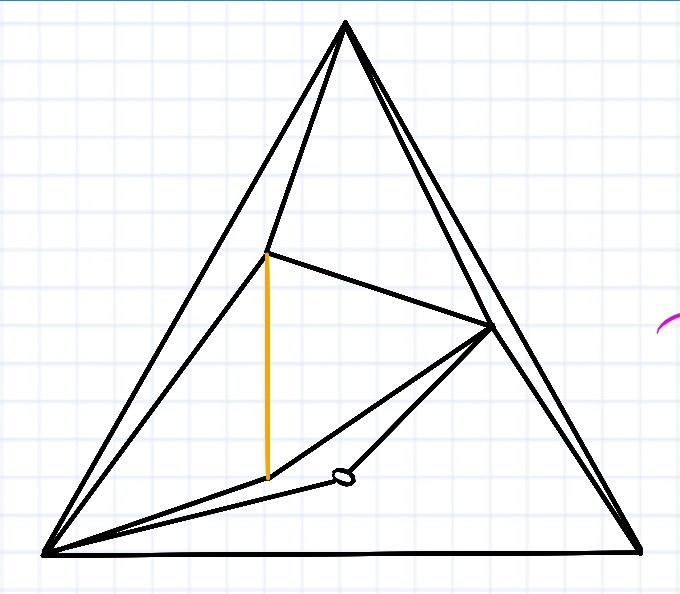
\includegraphics[width=0.5\linewidth]{drawings/two_triangles_1.jpg}
		\caption{Start the optimization here. The shortest edge is illustrated with an orange color}
	\end{subfigure}
	\begin{subfigure}{0.8\textwidth}
	\centering
	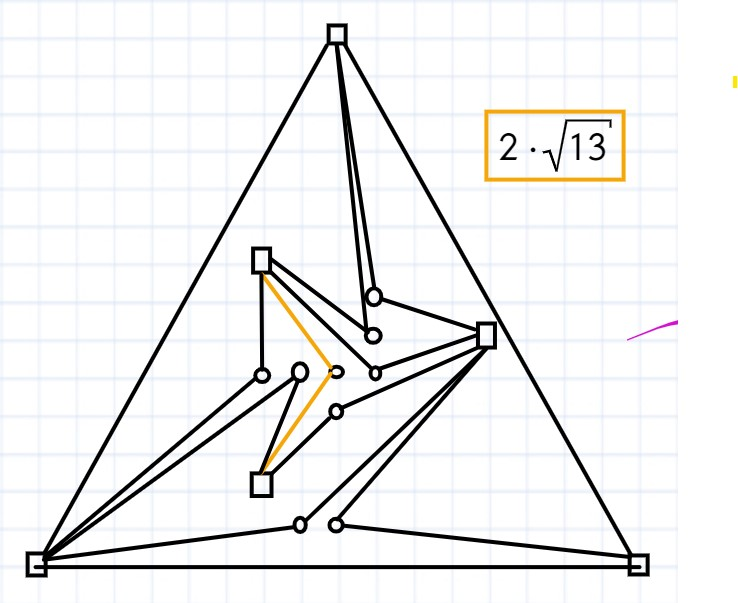
\includegraphics[width=0.5\linewidth]{drawings/two_triangles_2.jpg}
	\caption{Bends were included. The Unit Length equals the length of one box.}
\end{subfigure}
	\begin{subfigure}{0.8\textwidth}
	\centering
	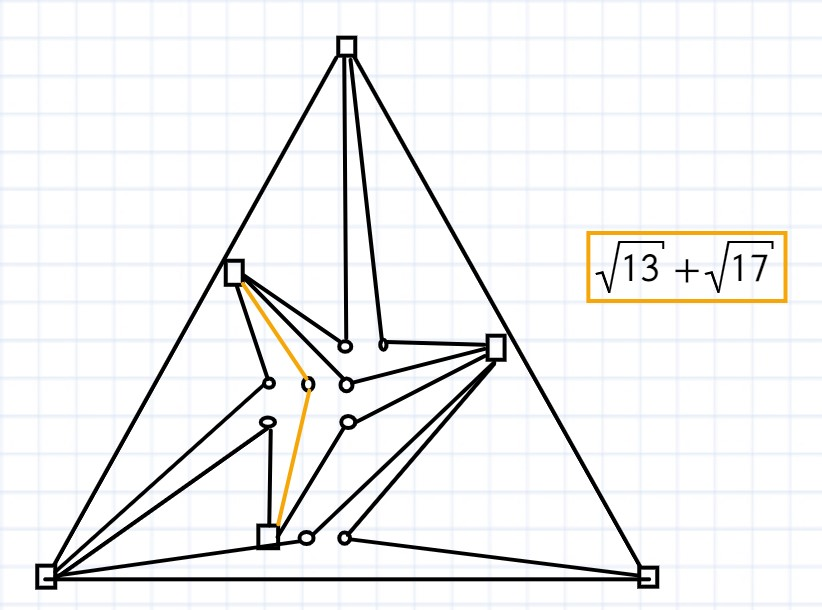
\includegraphics[width=0.5\linewidth]{drawings/two_triangles_3.jpg}
	\caption{Vertex and bend repositioned for a better result}
\end{subfigure}
	\begin{subfigure}{0.8\textwidth}
	\centering
	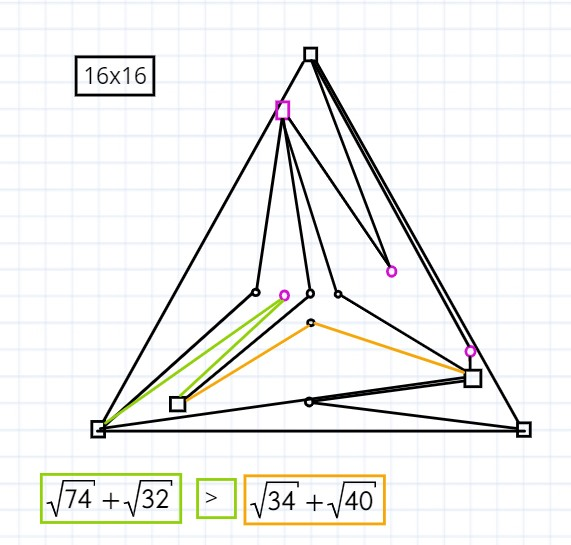
\includegraphics[width=0.5\linewidth]{drawings/two_triangles_4.jpg}
	\caption{After greedily elongate the shortest edge in a couple of iterations, it gets clear, how the triangles could be drawn with a satisfying ratio.}
\end{subfigure}
\end{figure}
This leads to the following approach, the discussion to the steps follow further below.
\begin{algorithm}[H]
	\KwIn{Graph consisting of $m$ triangles connected as illustrated above, Gridsize, one bend allowed}
	\KwOut{Drawing with a satisfying edge-length ratio}
	Draw the outermost triangle as big as possible on the grid with the approximated height\\
	\For{$i=2$ to $m$}{
		Place the $i$-th triangle inside the predecessor by a constant $c$\\
		Place bend points between those triangles and draw the edges with length bound by the shortest edge of the inner triangle and the longest edge of the outer triangle
	}
\caption{Algorithm sketch for a drawing of the example graph}
\end{algorithm}
Details:
\begin{enumerate}
	\item Recall the approximation for a uni-sized triangle of the first section for the triangle.
	\item It is important to have grid points between two consecutive triangle drawings. The bends must be placed somewhere.
	\item To get an idea, how exactly the bend points are set, please, take a look at the following picture.
	\begin{figure}[H]
		\centering
			\begin{subfigure}{0.8\textwidth}
			\centering
			\includegraphics[width=0.8\linewidth,page=7]{drawings/previous-results.pdf}
			\caption{This is the output of the algorithm with $m = 2$.}
		\end{subfigure}
		\begin{subfigure}{0.8\textwidth}
			\centering
			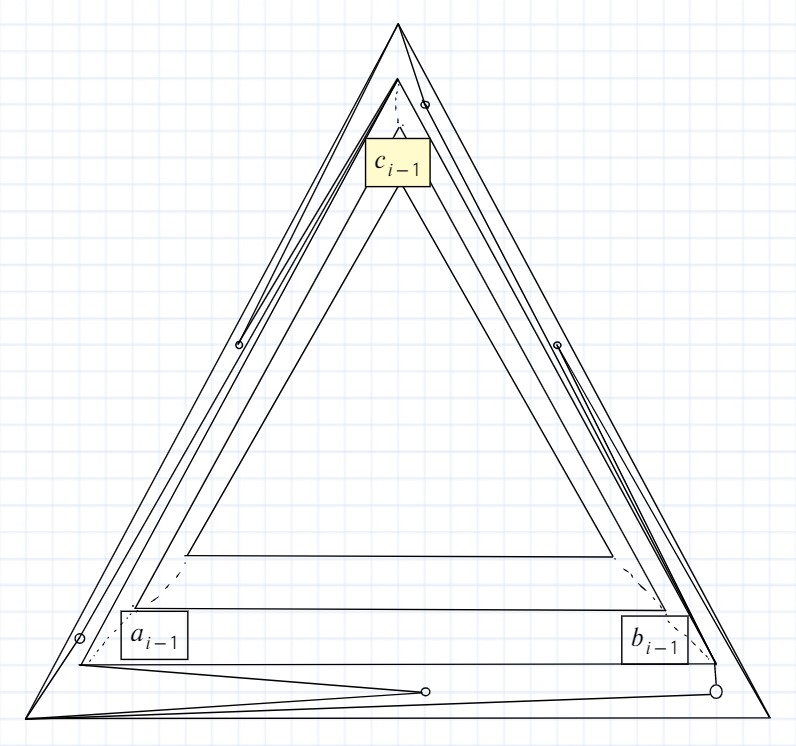
\includegraphics[width=0.8\linewidth]{drawings/variant_triangles_1.jpg}
			\caption{In this case, deg($a_1$)=5, deg($b_1$) = 3, deg($c_1$) = 4}
		\end{subfigure}

	\end{figure}
	The bend point for w.l.o.g. $(a_{i-1},a_i)$ lies centralized between $a_{i-1}, b_{i-1},a_i, b_i$. Analogue for the other ones. The bend point for w.l.o.g. $(a_{i-1},b_i$ lies below $b$. To guarantee the existence of those points, it is important not to choose the \grqq shrinking constant\grqq~$c$ too small.
\end{enumerate}
	\begin{lemma}
		With one bend allowed per edge, the graph above, inheriting $m$ triangles, will have an edge-length ratio in $\mathcal{O}(n)$.
	\end{lemma}
	\begin{proof}
		If the construction of the drawing is correct, then the innermost triangle $t_m$ will inherit the shortest edge and the outerface $t_1$ will contain the longest edge. Since the triangles have a constant distance pairwise, the differences between the edge lengths of the outermost and the innermost triangle is linear to the amount of triangles. Therefore, the ratio between the longest edge on the outermost triangle and the shortest edge on the innermost triangle grows linear with the amount of triangles. Hence, the ratio lies in $\mathcal{O}(n)$.
	\end{proof}
\subsection{Third example - a complete binary tree with depth $d$}
A binary tree is 1-connected. It is of interest, how the edge-length ratio behaves for a given depth $d$. In order to get a feeling, drawings of uniform long edges were created and it was observed, at which depth it is not possible to place further vertices.
\begin{observation}
	When the drawing starts with horizontal or vertical edges, it is not possible to draw a complete binary tree of depth $5$ with an edge-length ratio of 1.
\end{observation}
	\begin{figure}[H]
		\centering
		\begin{subfigure}{0.8\textwidth}
			\centering
			\includegraphics[width=0.5\linewidth,page=9]{drawings/Erste-Beispiele.pdf}
			\caption*{At some point, there is simply not enough area for $2^d$ vertices}
		\end{subfigure}
	\end{figure}
\begin{observation}
	If starting diagonally first, a complete binary tree of depth 5 is drawable on a 11x11 grid with a ratio of $\sqrt{2}$.
\end{observation}
	\begin{figure}[H]
	\centering
	\begin{subfigure}{0.8\textwidth}
		\centering
		\includegraphics[width=0.5\linewidth,page=9]{drawings/bintree-without-bends.jpg}
		\caption*{It seems that, when starting diagonally, there might be more grid points availiable}
	\end{subfigure}
\end{figure}
\begin{lemma}
	Allowing one bend, it is possible to draw a complete binary tree of depth $5$ with an edge-length ratio of 1.
\end{lemma}
\begin{proof}
		\begin{figure}[H]
		\centering
		\begin{subfigure}{0.8\textwidth}
			\centering
			\includegraphics[width=0.5\linewidth,page=9]{drawings/bintree-with-bends.jpg}
			\caption*{Using bends, all edges are of the same length}
		\end{subfigure}
	\end{figure}
\end{proof}
\begin{theorem}
	A complete binary tree with depth $d$ can be drawn with an edge-length ratio of $\mathcal{O}(\sqrt{n})$
\end{theorem}
\begin{proof}[Sketch of a proof]
	As already seen, for the depth up to 5, the edge-length ratio values 1. Incrementally, the drawing of $i$-th depth is achieved by copying the drawing of $i-1$ and each roots of the subtrees with a vertex. When looking at the drawing of depth $7$, then we observe that the ratio is the same as of the drawing with depth 6.
			\begin{figure}[H]
		\centering
		\begin{subfigure}{0.8\textwidth}
			\centering
			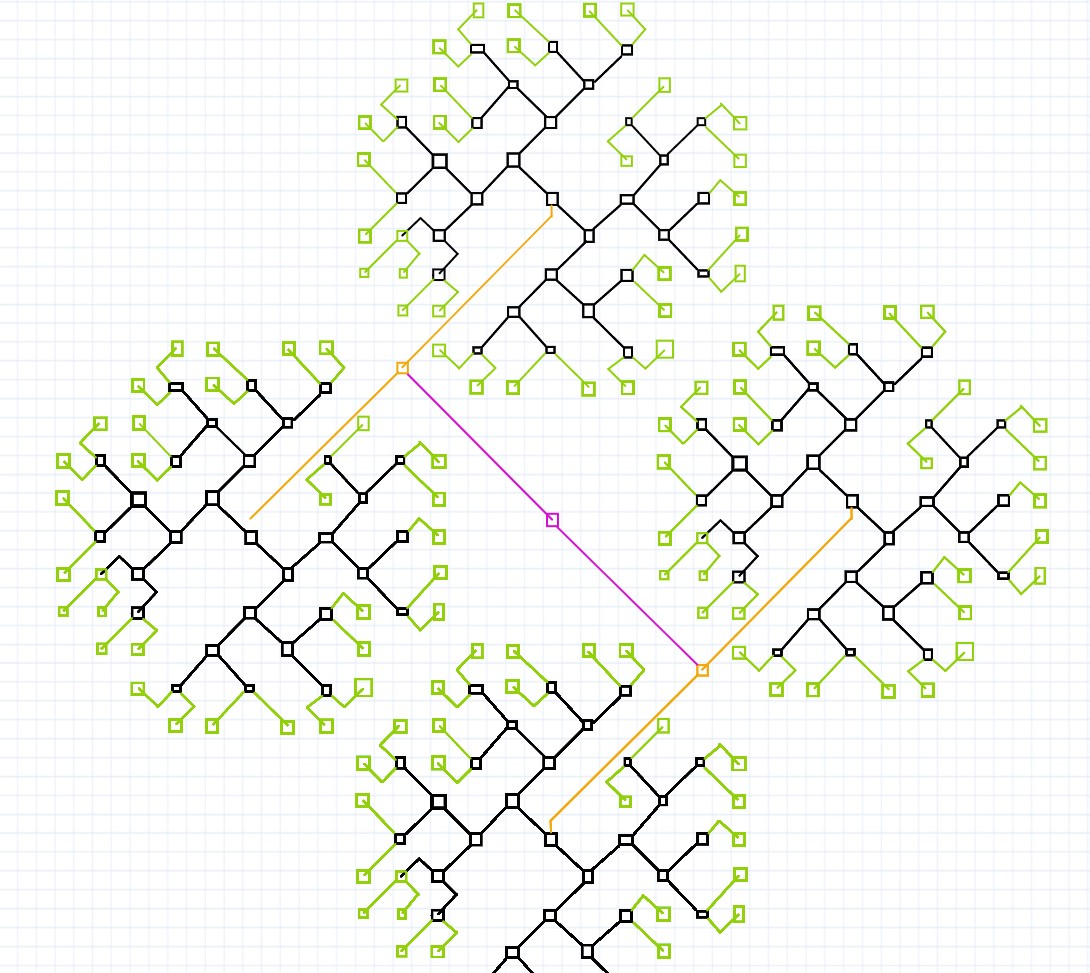
\includegraphics[width=\linewidth]{drawings/bintree-with-bends-depth-7.jpg}
			\caption*{Depth 6 in orange, depth 7 in purple}
		\end{subfigure}
	\end{figure}
	The ratio can be expressed as:
	\begin{align*}
		\text{ratio}_d = 2^{\lfloor\frac{d}{2}\rfloor-1} + \frac{1}{2}\in \mathcal{O}(\sqrt{n})
	\end{align*}
\end{proof}
\subsection{General observations / thoughts}
\begin{itemize}
	\item Draw large, thinking of one triangle
	\item \grqq twist\grqq a subgraph / component
	\item When components are nested, try to maintain a constant spacing
	\item Bend placement: either next to a vertex or in the center of a set of vertices
	\item Drawing diagonally is not a bad idea? (Binary tree)
	\item ???
\end{itemize}

\end{document}
